\subsection{Многомерные массивы}

Внутри многомерный массив выглядит так же как и линейный.

Ведь память компьютера линейная, это одномерный массив.
Но для удобства этот одномерный массив легко представить как многомерный.

К примеру, вот как элементы массива 3x4 расположены в одномерном массиве из 12 ячеек:

% TODO FIXME not clear. First, horizontal would be better. Second, why two columns?
% I'd first show 3x4 with numbered elements (e.g. 32-bit ints) in colored lines,
% then linear with the same numbered elements (and colored blocks)
% then linear with addresses (offsets) - assuming let say 32-bit ints.
\begin{table}[H]
\centering
\begin{tabular}{ | l | l | }
\hline
Смещение в памяти & элемент массива \\
\hline
0 & [0][0] \\
\hline
1 & [0][1] \\
\hline
2 & [0][2] \\
\hline
3 & [0][3] \\
\hline
4 & [1][0] \\
\hline
5 & [1][1] \\
\hline
6 & [1][2] \\
\hline
7 & [1][3] \\
\hline
8 & [2][0] \\
\hline
9 & [2][1] \\
\hline
10 & [2][2] \\
\hline
11 & [2][3] \\
\hline
\end{tabular}
\caption{Двухмерный массив представляется в памяти как одномерный}
\end{table}

Вот по каким адресам в памяти располагается каждая ячейка двухмерного массива 3*4:

\begin{table}[H]
\centering
\begin{tabular}{ | l | l | l | l | }
\hline                        
0 & 1 & 2 & 3 \\
\hline  
4 & 5 & 6 & 7 \\
\hline  
8 & 9 & 10 & 11 \\
\hline  
\end{tabular}
\caption{Адреса в памяти каждой ячейки двухмерного массива}
\end{table}

\myindex{row-major order}
Чтобы вычислить адрес нужного элемента, сначала умножаем первый индекс (строку) на 4 (ширину массива), 
затем прибавляем второй индекс (столбец).

Это называется \IT{row-major order}, 
и такой способ представления массивов и матриц используется по крайней мере в \CCpp и Python. 
Термин \IT{row-major order} означает по-русски примерно следующее: \q{сначала записываем элементы первой строки, затем второй,~\dots~и~элементы последней 
строки в самом конце}.

\myindex{column-major order}
\myindex{Фортран}
Другой способ представления называется \IT{column-major order} (индексы массива используются в обратном порядке) 
и это используется по крайней мере в Фортране, MATLAB и R. 
Термин \IT{column-major order} означает по-русски
следующее: \q{сначала записываем элементы первого столбца, затем второго,~\dots~и~элементы последнего столбца
в самом конце}.

Какой из способов лучше?
В терминах производительности и кэш-памяти, лучший метод организации данных это тот,
при котором к данным обращаются последовательно.

Так что если ваша функция обращается к данным построчно, то \IT{row-major order} лучше,
и наоборот.

% subsections
\subsubsection{Пример с двумерным массивов}

Мы будем работать с массивом типа \Tchar. Это значит, что каждый элемент требует
только одного байта в памяти.

\myparagraph{Пример с заполнением строки}
\myindex{\olly}

Заполняем вторую строку значениями 0..3:

\lstinputlisting[caption=Пример с заполнением строки,style=customc]{patterns/13_arrays/5_multidimensional/two1_RU.c}

Все три строки обведены красным. 
Видно, что во второй теперь имеются байты 0, 1, 2 и 3:

\begin{figure}[H]
\centering
\includegraphics[width=0.6\textwidth]{patterns/13_arrays/5_multidimensional/olly_2D_1.png}
\caption{\olly: массив заполнен}
\end{figure}

\myparagraph{Пример с заполнением столбца}
\myindex{\olly}

Заполняем третий столбец значениями 0..2:

\lstinputlisting[caption=Пример с заполнением столбца,style=customc]{patterns/13_arrays/5_multidimensional/two2_RU.c}

Здесь также обведены красным три строки. 
Видно, что в каждой строке, на третьей позиции, теперь записаны 0, 1 и 2.

\begin{figure}[H]
\centering
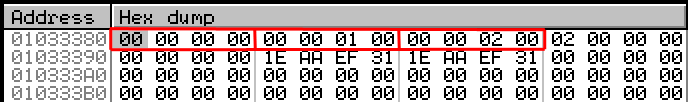
\includegraphics[width=0.6\textwidth]{patterns/13_arrays/5_multidimensional/olly_2D_2.png}
\caption{\olly: массив заполнен}
\end{figure}

\subsubsection{Работа с двухмерным массивом как с одномерным}

Мы можем легко убедиться, что можно работать с двухмерным массивом как с одномерным,
используя по крайней мере два метода:

\lstinputlisting[style=customc]{patterns/13_arrays/5_multidimensional/2D_as_1D_RU.c}

Компилируете и запускаете: мы увидим корректные значения.

Очарователен результат работы MSVC 2013~--- все три процедуры одинаковые!

\lstinputlisting[caption=\Optimizing MSVC 2013 x64,style=customasmx86]{patterns/13_arrays/5_multidimensional/2D_as_1D_MSVC_2013_Ox_x64_RU.asm}

GCC сгенерировал практически одинаковые процедуры:

\lstinputlisting[caption=\Optimizing GCC 4.9 x64,style=customasmx86]{patterns/13_arrays/5_multidimensional/2D_as_1D_GCC49_x64_O3_RU.s}


\subsubsection{Пример с трехмерным массивом}

То же самое и для многомерных массивов.
На этот раз будем работать с массивом типа \Tint: каждый элемент требует 4 байта в памяти.

Попробуем:

\lstinputlisting[caption=простой пример,style=customc]{patterns/13_arrays/5_multidimensional/multi.c}

\myparagraph{x86}

В итоге (MSVC 2010):

\lstinputlisting[caption=MSVC 2010,style=customasmx86]{patterns/13_arrays/5_multidimensional/multi_msvc_RU.asm}

В принципе, ничего удивительного. В \TT{insert()} для вычисления адреса нужного элемента массива 
три входных аргумента перемножаются по формуле $address=600 \cdot 4 \cdot x + 30 \cdot 4 \cdot y + 4z$, 
чтобы представить массив трехмерным.
Не забывайте также, что тип \Tint 32-битный (4 байта), поэтому все коэффициенты нужно умножить на 4.

\lstinputlisting[caption=GCC 4.4.1,style=customasmx86]{patterns/13_arrays/5_multidimensional/multi_gcc_RU.asm}

Компилятор GCC решил всё сделать немного иначе.
Для вычисления одной из операций ($30y$), GCC создал код, где нет самой операции умножения.

Происходит это так: 
$(y+y) \ll 4 - (y+y) = (2y) \ll 4 - 2y = 2 \cdot 16 \cdot y - 2y = 32y - 2y = 30y$. 
Таким образом, для вычисления $30y$ используется только операция сложения, 
операция битового сдвига и операция вычитания.
Это работает быстрее.

\myparagraph{ARM + \NonOptimizingXcodeIV (\ThumbMode)}

\lstinputlisting[caption=\NonOptimizingXcodeIV (\ThumbMode),style=customasmARM]{patterns/13_arrays/5_multidimensional/multi_Xcode_thumb_O0_RU.asm}

\NonOptimizing LLVM сохраняет все переменные в локальном стеке, хотя это и избыточно.

Адрес элемента массива вычисляется по уже рассмотренной формуле.

\myparagraph{ARM + \OptimizingXcodeIV (\ThumbMode)}

\lstinputlisting[caption=\OptimizingXcodeIV (\ThumbMode),style=customasmARM]{patterns/13_arrays/5_multidimensional/multi_Xcode_thumb_O3_RU.asm}

Тут используются уже описанные трюки для замены умножения на операции сдвига, сложения и вычитания.

\myindex{ARM!\Instructions!RSB}
\myindex{ARM!\Instructions!SUB}
Также мы видим новую для себя инструкцию \RSB (\IT{Reverse Subtract}).
Она работает так же, как и \SUB, только меняет операнды местами.

Зачем?
\myindex{ARM!Optional operators!LSL}
\SUB и \RSB это те инструкции, ко второму операнду которых можно применить коэффициент сдвига, как мы видим и здесь: (\INS{LSL\#4}). 
Но этот коэффициент можно применить только ко второму операнду.

Для коммутативных операций, таких как сложение или умножение, 
операнды можно менять местами и это не влияет на результат.

Но вычитание~--- операция некоммутативная, так что для этих случаев существует инструкция \RSB.

\myparagraph{MIPS}

\myindex{MIPS!Global Pointer}

Мой пример такой крошечный, что компилятор GCC решил разместить массив $a$ в 64KiB-области,
адресуемой при помощи Global Pointer.

\lstinputlisting[caption=\Optimizing GCC 4.4.5 (IDA),style=customasmMIPS]{patterns/13_arrays/5_multidimensional/multi_MIPS_O3_IDA_RU.lst}



\subsubsection{Ещё примеры}

Компьютерный экран представляет собой двумерный массив, но видеобуфер это линейный
одномерный массив. 
Мы рассматриваем это здесь: \myref{Mandelbrot_demo}.

Еще один пример в этой книге это игра ``Сапер'': её поле это тоже двухмерный массив: \ref{minesweeper_winxp}.

